% Overview of the closed loop (fig:overview), single column, vertical.
% Build:  cd figures && pdflatex overview-loop.tex   (or: make figure-overview)
% Panels are cropped by scripts/figures/build_overview_photos.py and
% scripts/figures/build_design_space_figure.py into photos/overview/;
% provenance of every photograph is in photos/README.md.
% Frames and arrows are grayscale; only the photographs carry color.
\documentclass[tikz,border=1pt]{standalone}
\usepackage{graphicx}
\usetikzlibrary{arrows.meta,positioning,calc,fit}

\newcommand{\pic}[2]{\includegraphics[height=#1]{photos/overview/#2}}
\newcommand{\piccap}[1]{{\tiny\textcolor{black!70}{#1}}}

\begin{document}
\begin{tikzpicture}[
  font=\sffamily\scriptsize,
  frame/.style={draw=black!45, line width=0.6pt, inner sep=2.2pt,
                text width=79mm, align=center},
  title/.style={anchor=north west, font=\sffamily\small, inner sep=0pt},
  flow/.style={-{Latex[length=2.2mm]}, line width=0.9pt, draw=black!70},
  back/.style={-{Latex[length=2.2mm]}, line width=0.8pt, draw=black!60,
               dash pattern=on 3pt off 2pt},
]
  % ---- Initialize ---------------------------------------------------------
  \node[frame] (init) {%
    \parbox[c]{79mm}{\raggedright\textbf{Initialize}
      \textcolor{black!55}{campaign}}\\[1pt]
    \pic{19mm}{initialize-design-space.pdf}\hspace{3mm}%
    \parbox[b]{22mm}{\raggedright\piccap{five continuous geometry variables;
      a Sobol seed batch of nine designs}}};

  % ---- Design (proposal BO panel, unchanged) ------------------------------
  \node[frame, below=4mm of init] (design) {%
    \parbox[c]{79mm}{\raggedright\textbf{Design}
      \textcolor{black!55}{experiments}}\\[1pt]
    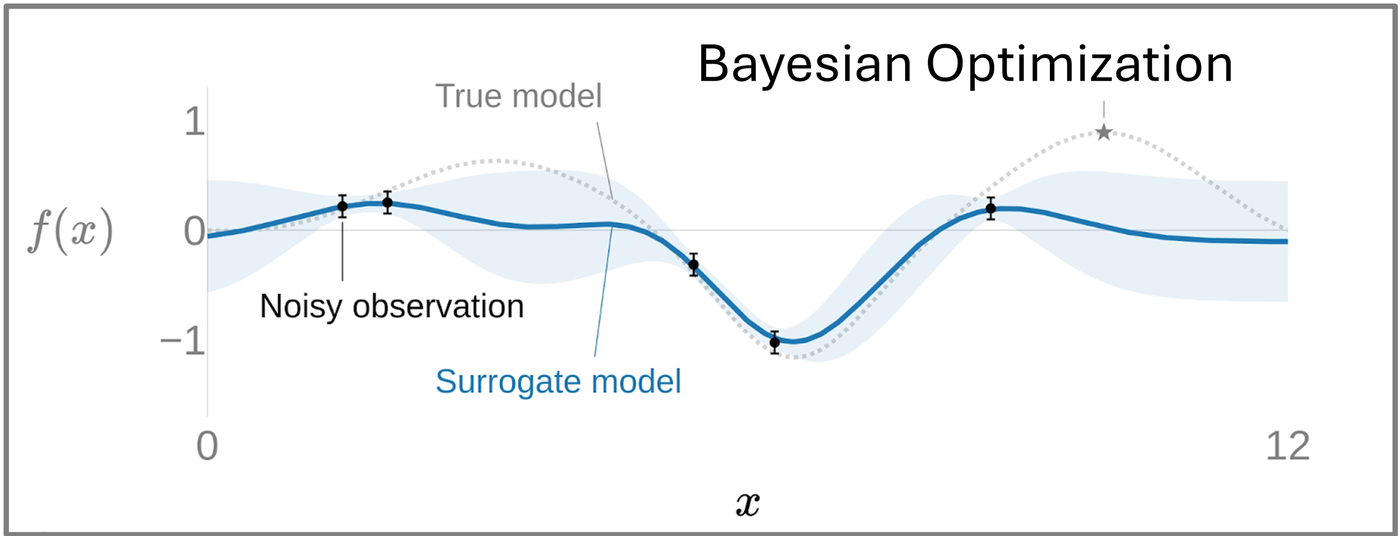
\includegraphics[width=62mm]{photos/overview/design-bo-panel.png}};

  % ---- Make ----------------------------------------------------------------
  \node[frame, below=4mm of design] (make) {%
    \parbox[c]{79mm}{\raggedright\textbf{Make}
      \textcolor{black!55}{specimens}}\\[1pt]
    \begin{tabular}{@{}c@{\hspace{1.2mm}}c@{\hspace{1.2mm}}c@{}}
      \pic{18.5mm}{make-plate-render.jpg} &
      \pic{18.5mm}{make-painted-supports.jpg} &
      \pic{18.5mm}{make-h2d-midprint.jpg} \\[-0.5pt]
      \piccap{batch-4 plate}
      & \piccap{painted supports}
      & \piccap{H2D mid-print}
    \end{tabular}};

  % ---- Test ----------------------------------------------------------------
  \node[frame, below=4mm of make] (test) {%
    \parbox[c]{79mm}{\raggedright\textbf{Test}
      \textcolor{black!55}{performance}}\\[1pt]
    \begin{tabular}{@{}c@{\hspace{1.2mm}}c@{}}
      \pic{21mm}{test-taped-batch.jpg} &
      \pic{21mm}{test-carriage.jpg} \\[-0.5pt]
      \piccap{labeled batch}
      & \piccap{specimen on the drop carriage}
    \end{tabular}};

  % ---- Conclude --------------------------------------------------------------
  \node[frame, below=4mm of test] (conclude) {%
    \parbox[c]{79mm}{\raggedright\textbf{Conclude}
      \textcolor{black!55}{campaign}\quad
      {\tiny\textcolor{black!70}{report the final Pareto front}}}};

  % ---- arrows ----------------------------------------------------------------
  \draw[flow] (init.south) -- (design.north);
  \draw[flow] (design.south) -- (make.north);
  \draw[flow] (make.south) -- (test.north);
  \draw[flow] (test.south) -- (conclude.north);
  % dashed return from Test back up to Design, outside the left edge
  \draw[back] (test.west) -- ++(-3.2mm,0) |- (design.west);
\end{tikzpicture}
\end{document}
